\documentclass[12pt]{article}
\usepackage{parskip}
\usepackage{amsmath}
\usepackage{pdfpages}
\usepackage{listings}
\usepackage{color}
\usepackage[margin=.6in]{geometry}

\definecolor{dkgreen}{rgb}{0,0.6,0}
\definecolor{gray}{rgb}{0.5,0.5,0.5}
\definecolor{mauve}{rgb}{0.58,0,0.82}

\lstset{frame=tb,
  language=C++,
  aboveskip=3mm,
  belowskip=3mm,
  showstringspaces=false,
  columns=flexible,
  basicstyle={\small\ttfamily},
  numbers=none,
  numberstyle=\tiny\color{gray},
  keywordstyle=\color{blue},
  commentstyle=\color{dkgreen},
  stringstyle=\color{mauve},
  breaklines=true,
  breakatwhitespace=true,
  tabsize=3
}
\begin{document}
\includepdf[pages=3]{slides.pdf}
We  want to use heuristics to make our life better. By either loosening the bounds or ensure that the solution is complete. We can use a heuristic to define how close you are to a goal. We call this the estimated cost. 

\includepdf[pages=4-6]{slides.pdf}
Say we have some initial state. From there we can create all possible moves. From there we can evaluate which move is most beneficial by using this cost heuristic to see how close that possibility is to the solution we want. 

\includepdf[pages=7]{slides.pdf}
A hill climbing algorithm is a iterative algorithm that starts with a solution to the problem and then tries to improve it. We come up with a bunch of children solutions and sort them based on the heuristic. If some change produces a better solution we repeat all of this on that solution. For the travelling salesman problem we can get some solution and then try stuff like switching the order of two cities and such. Eventually we will find a much shorter route.

\includepdf[pages=9]{slides.pdf}
We always want our successors to have a smaller cost (meaning that they are more optimal). We will chose a successor that is better than the current solution and better than all other possible successors. There is no back tracking here. 

\includepdf[pages=13-14]{slides.pdf}
Here we only look a little bit ahead when deciding which way to go. We compare all things to a depth of 2. We only find the best two children and go on those. So we look at B and C and see that C is better so we go there. From there we look at F and G and find that F is better. 

LOOK MORE INTO THIS

\includepdf[pages=15]{slides.pdf}
When we look at the successors of a node to the expanded list. We can then sort based on heuristic and go from there. When you are at A, look at B and C, C is better so you go there. Look at its children. While you can find a better solution keep going deeper, choosing the most promising children as you go. Basically this is just a greedy search. 

\includepdf[pages=17-18]{slides.pdf}
Here we want to eliminate paths that hold no promise. We calculate the cost from the start to you (g(n)) and the estimated cost from you to the end (h(n)). So we total these to get the promise of a node. We want to use an admissible heuristic.

\includepdf[pages=19]{slides.pdf}
An admissible heuristic never overestimates the cost of getting to the goal. We never want to discount a good solution by overestimating its cost.

\includepdf[pages=20]{slides.pdf}
We look at how many misplaced tiles there are. We know that this is admissible because each of those misplaced tiles must be moved at least once so this cost will be less than the actual cost.

\includepdf[pages=22]{slides.pdf}
We can come up with heuristics by relaxing rules for the game. 

LOOK MORE INTO THIS: \url{https://en.wikipedia.org/wiki/Admissible_heuristic}

\includepdf[pages=26]{slides.pdf}
For every move by everyone you label each one. You want yours to be maximal and they want yours to be minimal. You have to generate all of these possibilities an analyse the best movements. There is a tone of possibilities so we want to try to simplify things. We can use this to predict what they will do and figure out how the game will go.

\includepdf[pages=30]{slides.pdf}
We define b to represent the average branching factor and d to be the average depth. These numbers are used to calculate the average number of possibilities ($b^d$). Instead of enumerating all possibilities we want to try to come up with an evaluation function that does not require looking ahead into future possibilities. For the tick tack toe example you could enumerate the number of possible wins not blocked for you minus the number of wins not blocked for them.

\includepdf[pages=45]{slides.pdf}
Alpha Beta pruning assumes that eveyone is going to make optimal moves so we can eliminate all of those branches that are not maximal.

\includepdf[pages=56]{slides.pdf}
Meta-hueristics try to go into higher levels. Basically we start looking at heuristics for heuristics. They are two types, tragectory and population.

\begin{itemize}
  \item Tragectory: looks at one solution at a time and back tracks how to get there
  \item Population: looks at multiple solutions
\end{itemize}









\end{document}